\documentclass[dutch]{report}
\usepackage[utf8]{inputenc}
\usepackage{babel}

\usepackage{titling}
\usepackage{graphicx}
\usepackage[utf8]{inputenc}

\usepackage{internship-docs-styling/style/a4-document-setup}
\usepackage{internship-docs-styling/style/internship-styling}

\author{Mies van der Lippe \& Roel Huizing}
\title{IKPMD I StayConnected App}

\renewcommand{\versiondate}{10-04-2020}
\renewcommand{\versionnumber}{0.1.0}
\renewcommand{\versionname}{Finalversie}


\usepackage{listings}
\usepackage{enumitem}

\begin{document}
	
	\begin{titlepage}
	
	\stylizedtitle
	\stylizedauthor
	\titlepageversion
	
	\vfill
	
	\begin{tabular}{rl}
		Student 1 & Mies van der Lippe \hspace{1cm}S1096607\\
		Student 2 & Roel Huizing \hfill S1092755\\
		Vak		  & IKPMD \\
	\end{tabular}
	
	\vspace{10mm}
	
	\hfill
	\includegraphics[height=1.5cm]{internship-docs-styling/img/hsl.png}	
	
\end{titlepage}
	\tableofcontents

	\newpage
	
	\section{Inleiding}
	Dit document omschrijft de app die Roel en Mies ontwikkeld hebben voor IKPMD. Het is een app waarin evenementen georganiseerd kunnen worden. 
	
	Het eerste hoofdstuk gaat over de functionaliteit en het functioneren van de app. Met allerlei screenshots en uitleg word behandeld hoe de 
	app gebruikt kan worden. Het eerste hoofdstuk legt ook uit welke middelen gebruikt zijn, en wat de performance van de app is. 
	
	In het hoofdstuk over Design wordt uitgelegd waarom sommige keuzes gemaakt zijn. Er is dicht bij de richtlijnen van Google gebleven en 
	het resultaat is een overzichtelijke app ontwikkeld. Dat is niet om te zeggen dat het saai is, het tegendeel wordt in dat hoofdstuk bewezen. 
	
	Dan volgt een technisch verhaal over hoe gegevens in de app tot stand komen. Er bestond al een website van de organisatie, maar nu is er ook 
	een API gebouwd. Gegevens uit de app worden op slimme wijze bewaard. 
	
	In Eigen Inbreng wordt uitgelegd wat de groep gedaan heeft dat niet binnen de normale opdracht valt. Het blijkt dat het misschien zelfs wel een
	tikkie minder gekund had, op een na worden alle voorbeelden benoemd. 
	
	Opvolgend is de omschrijving van het versiebeheer. Daarop volgt een bronnenlijst. 
	
	Als laatste onderdeel van dit document volgt de reflectie en de individuele inleg van de groepsleden. 
	
	\subsection{Wat is StayConnected eigenlijk?}
	Stayconnected is een initiatief van ExPex. Dit is een organisatie die zich bezighoud met mensen die in contact zijn (geweest) met jeugdhulp. Zij 
	zetten zich dus in voor (voormalig) jongeren die hulp krijgen of hebben gehad. Omdat het vaak gaat over onderwerpen waar wij leken weinig van 
	kunnen snappen, organiseert StayConnected bijeenkomsten voor jongeren die inmiddels uit het traject zijn. Zij kunnen dan praten met mensen 
	die zij kennen uit hun behandeling, of die hen begrijpen. 
	
	\newpage
	
	\section{Productverslag}
	De app die gemaakt is is als het ware een interface voor het werken met de achterliggende API.
	In de app is het mogelijk om te authenticeren met de API door middel van het login scherm, evenementen bekijken die ook op de website te zien zijn en evenementen aanmaken.
		
	\begin{minipage}{0.33\textwidth}
		\begin{center}
			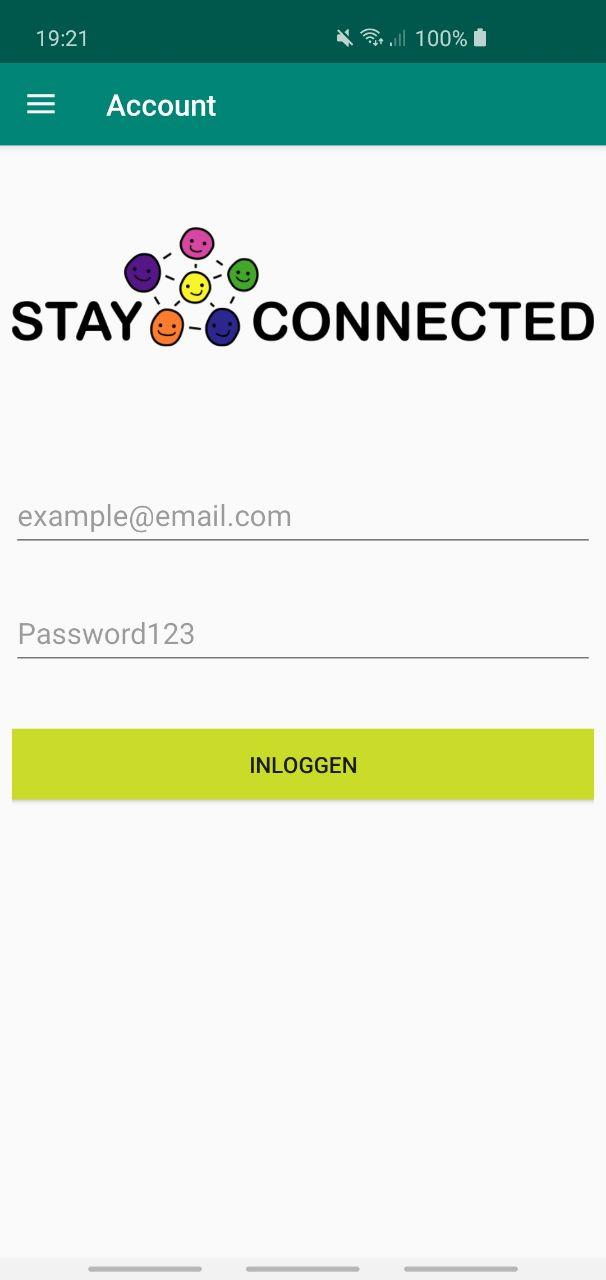
\includegraphics[width=3cm]{images/FOTOLOGINSCHERM.jpg}		
		\end{center}
	\end{minipage}
	\begin{minipage}{0.34\textwidth}
		\begin{center}
			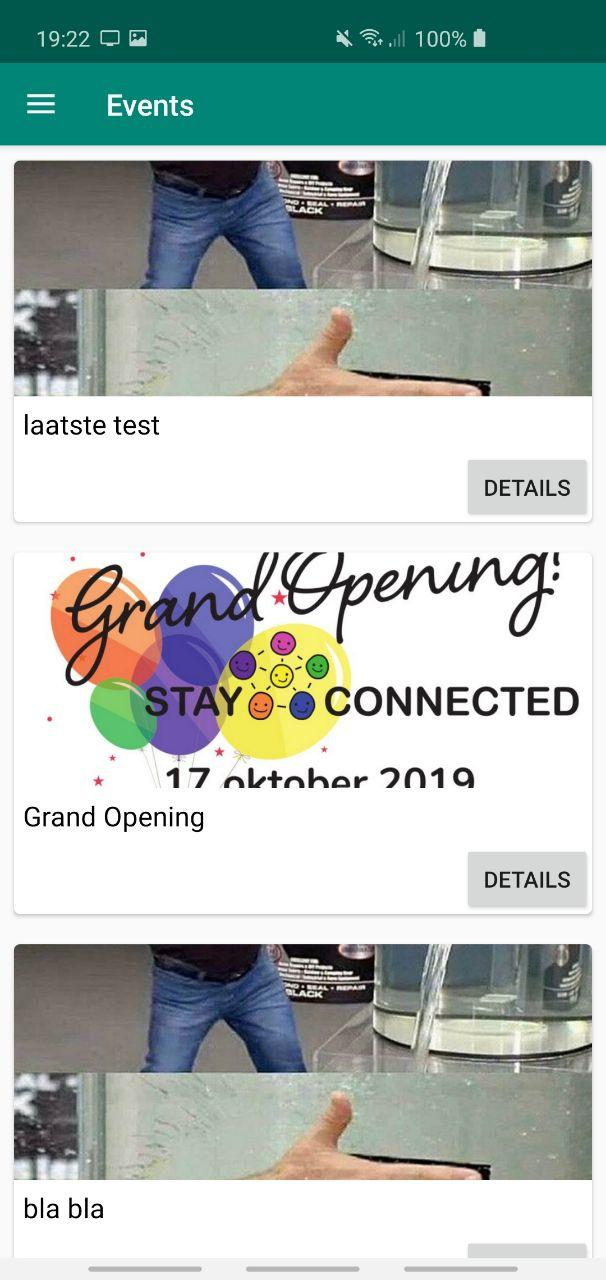
\includegraphics[width=3cm]{images/FOTOEVENTLIJST.jpg}
		\end{center}
	\end{minipage}
	\begin{minipage}{0.33\textwidth}
		\begin{center}
			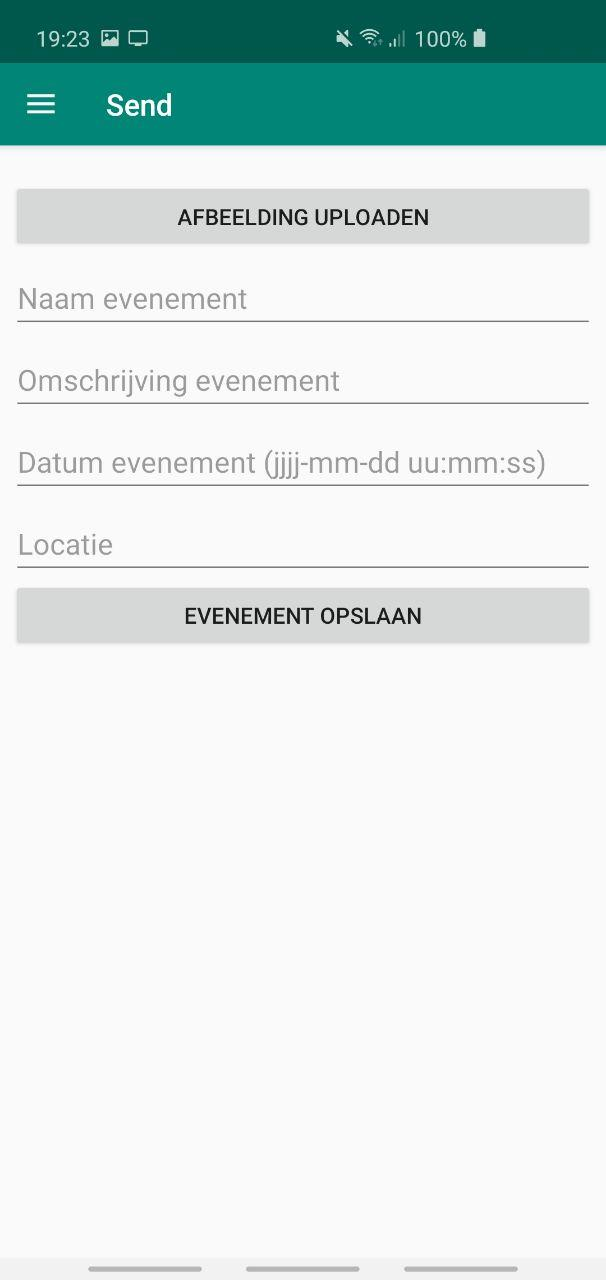
\includegraphics[width=3cm]{images/FOTOEVENTCREATE.jpg}
		\end{center}
	\end{minipage}
	
	Als er op de login-knop gedrukt wordt zonder dat het emailadres wat is gegeven valide is, wordt er een error bericht laten zien.
	
	Op het moment dat een gebruiker inlogd, wordt er een POST request gestuurd naar de API met het email en wachtwoord. De API geeft vervolgens,
	bij een succesvolle login, een token terug wat voor verdere authenticatie gebruikt wordt binnen de app en om verdere userdata zoals: naam en geboortedatum
	op te halen van de API.
	Deze token wordt ook opgeslagen in een private SharedPreference, samen met de naam van de gebruiker, email, en admin status om de login persistent te maken
	,en te zorgen voor persoonlijke UI elementen, zoals het laten zien van de gebruikersnaam in de drawer 
	Wanneer iemand niet in ingelogd staat er op de plek van de gebruikersnaam dat de gebruiken niet is ingelogd en kan inloggen in het Account menu. 
	
	\begin{minipage}{0.33\textwidth}
		\begin{center}
			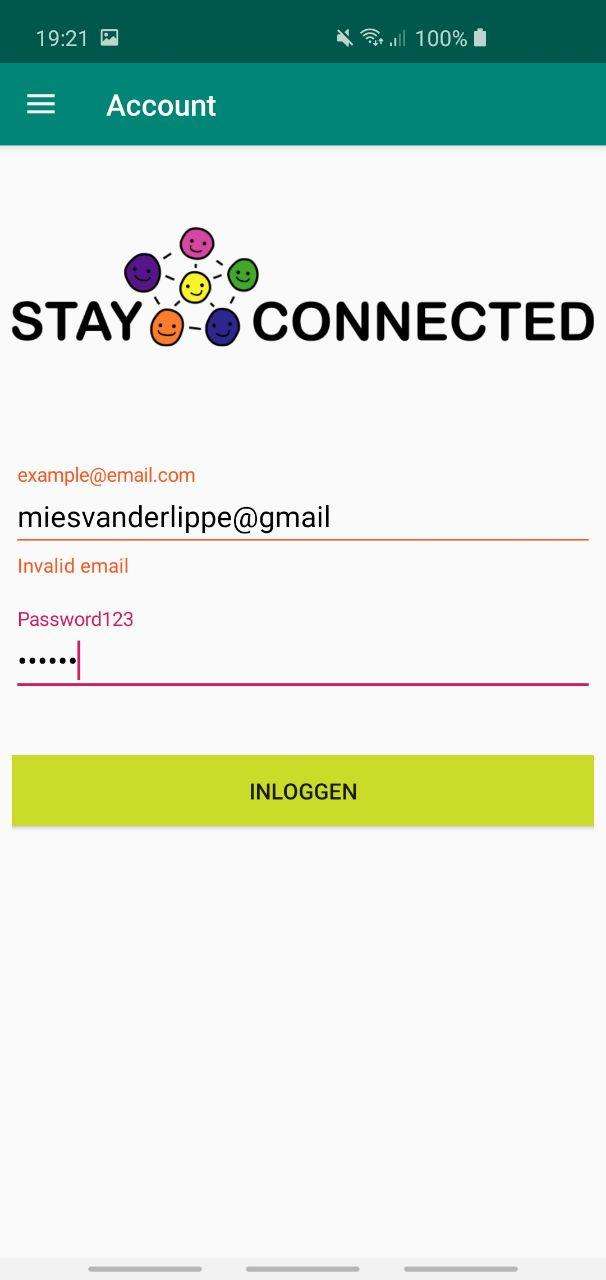
\includegraphics[width=3cm]{images/FOTOINVALIDEMAIL.jpg}		
		\end{center}
	\end{minipage}
	\begin{minipage}{0.34\textwidth}
		\begin{center}
			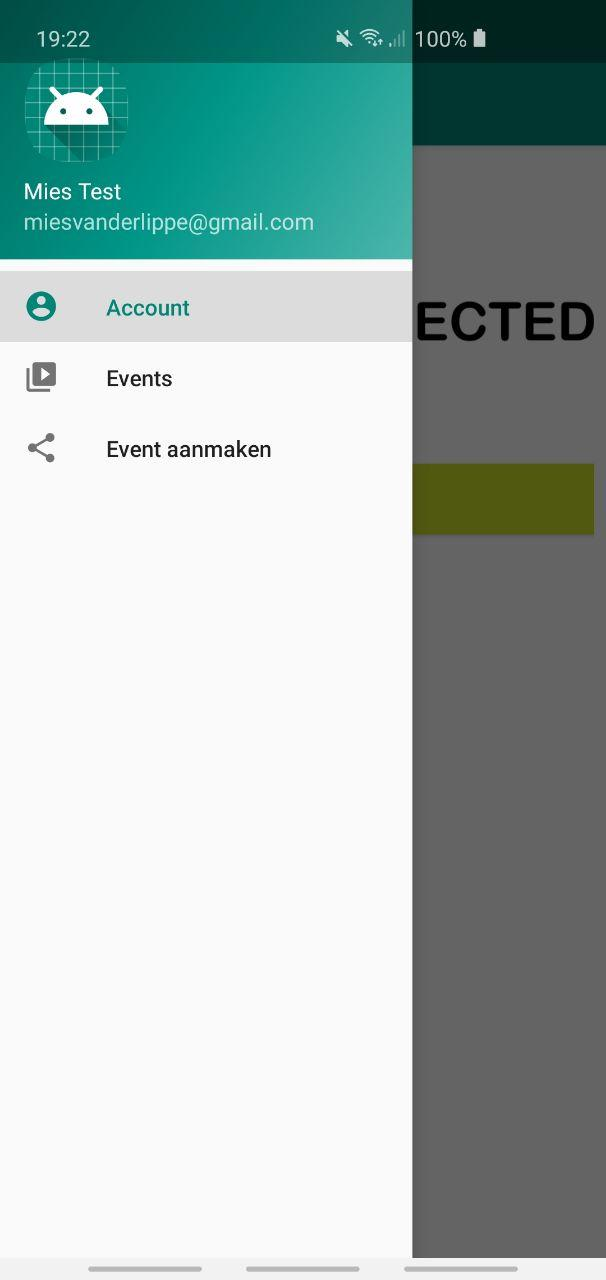
\includegraphics[width=3cm]{images/FOTONAAMINDRAWER.jpg}
		\end{center}
	\end{minipage}
	\begin{minipage}{0.33\textwidth}
		\begin{center}
			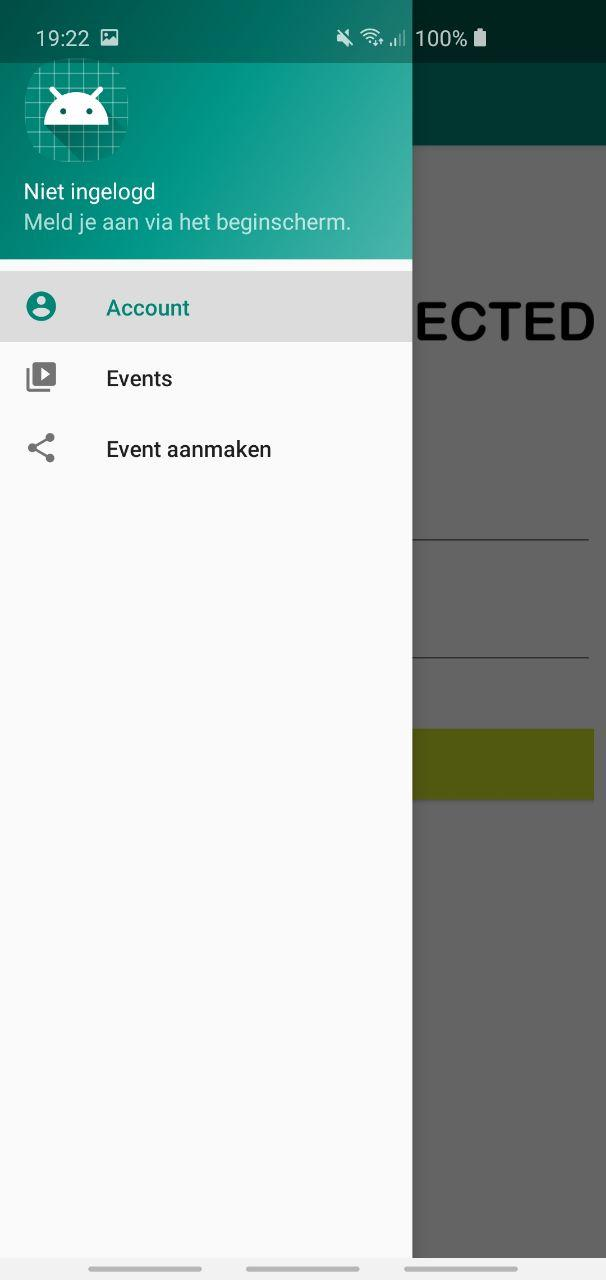
\includegraphics[width=3cm]{images/FOTOGEENNAAMINDRAWER.jpg}
		\end{center}
	\end{minipage}
	
	Op het moment is voor het maken van evenementen alleen een valide login nodig. Wanneer de gebruiker niet is ingelogd kan hij geen evenementen aanmaken en krijgt dat te zien. 
	Wanneer een gebruiker is ingelogd kan hij een evenement aanmaken. Een evenement heeft een aantal vereisten: een naam, beschrijving, datum en een locatie. Een foto kan ook worden meegegeven,
	hoewel dit niet verplicht is.  Als de gebruiker vervolgens op de knop "Evenement aanmaken" drukt, wordt er een POST request naar de API gestuurd met de opties in de 
	request body. Als het maken van het evenement succesvol is, wordt een toast zichtbaar waarin staat dat het evenement is aangemaakt. 
	
	\begin{minipage}{0.33\textwidth}
		\begin{center}
			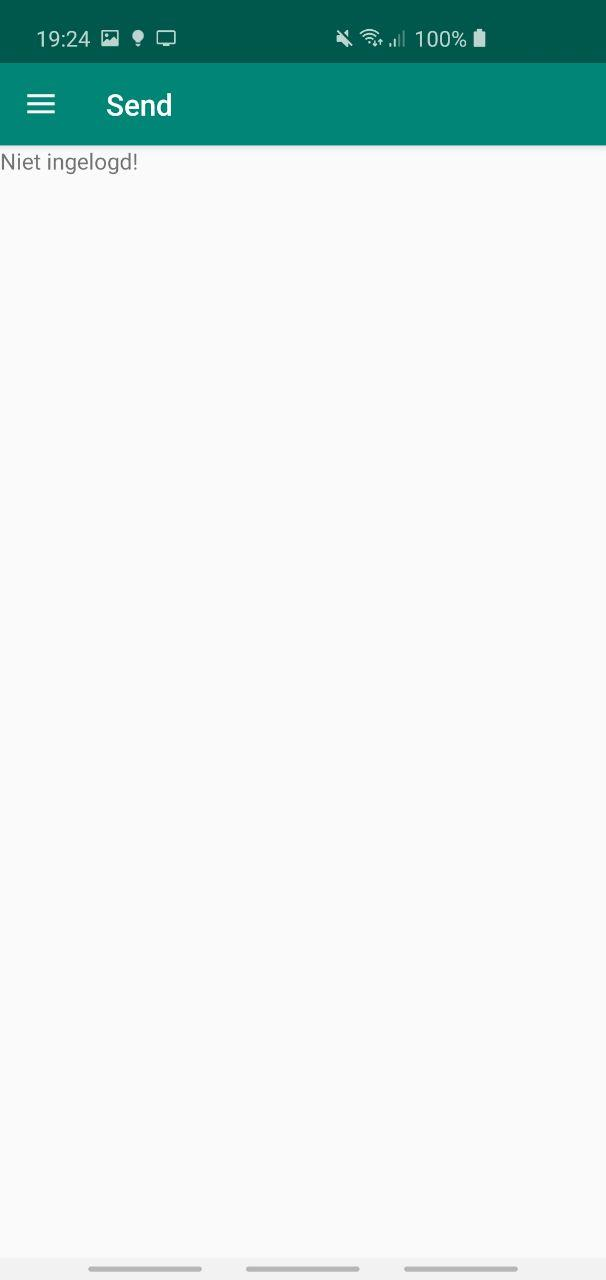
\includegraphics[width=3cm]{images/FOTOKANGEENEVENTMAKEN.jpg}		
		\end{center}
	\end{minipage}
	\begin{minipage}{0.34\textwidth}
		\begin{center}
			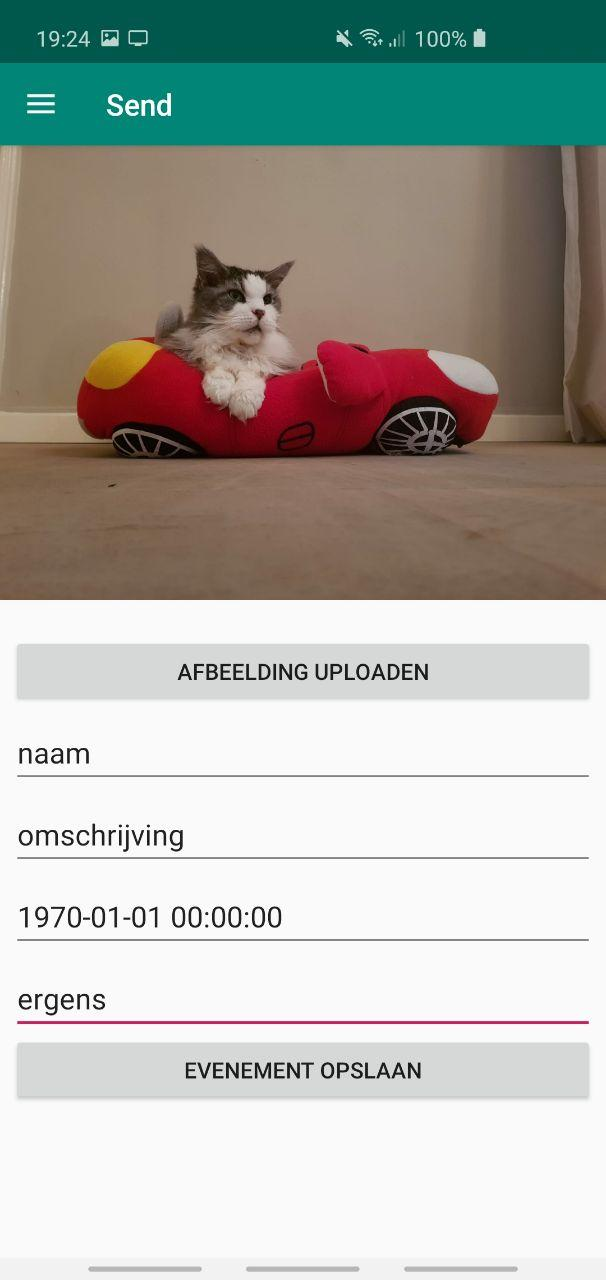
\includegraphics[width=3cm]{images/FOTOINGEVULDEVENT.jpg}
		\end{center}
	\end{minipage}
	\begin{minipage}{0.33\textwidth}
		\begin{center}
			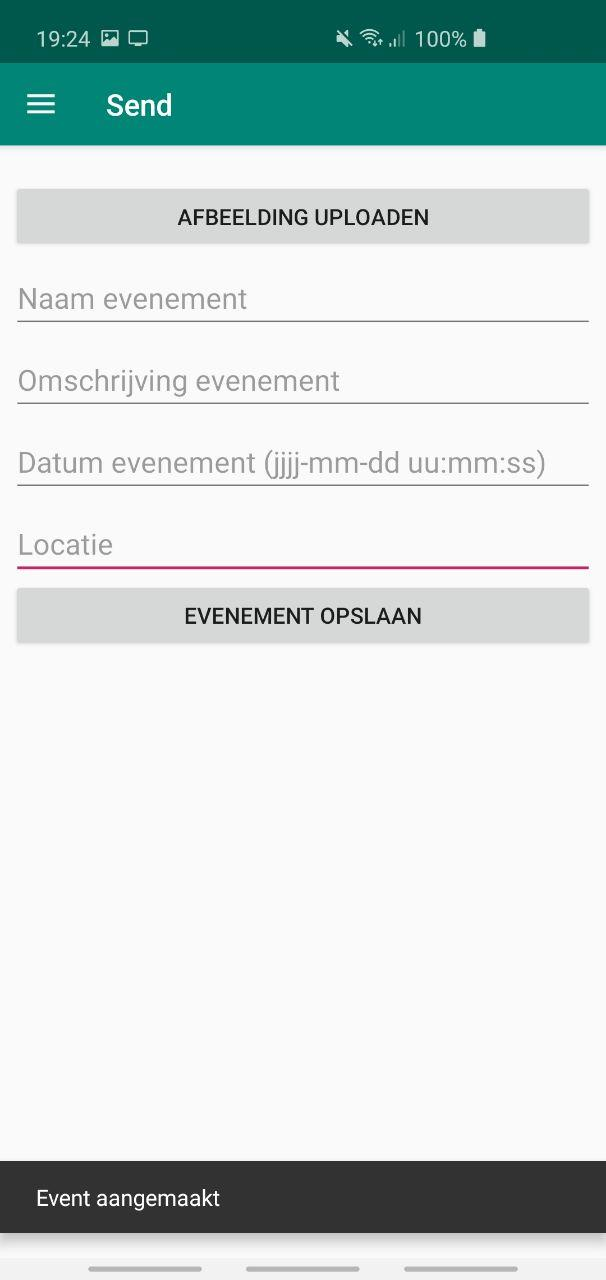
\includegraphics[width=3cm]{images/FOTOEVENTAANGEMAAKT.jpg}
		\end{center}
	\end{minipage}
	
	Nadat het evenement gemaakt is, is deze gelijk te zien onder "Events". 
	Details over een specifiek evenement zijn te zien wanneer de gebruiker op "Details" drukt onder een event.
	Voor het bekijken van evenementen is geen login vereist. Elke gebruiker van de app kan de lijst met evenementen zien.
	
	\subsection{Build opties}
	De ontwikkelde app is gemaakt met gebruik van Android SDK 29, sinds dat dit de meest recente versie van de SDK is op het moment van ontwikkeling.
	Bij het ontwikkelen is er gebruik gemaakt van Gradle, waarbij een aantal aanpassingen gemaakt zijn. De aanpassingen zijn  een aantal dependencies, deze zijn:
	 \begin{enumerate}
	 	\item Volley: Voor het maken van HTTP requests
	 	\item Gson: Voor het converteren van JSON data naar java objecten en andersom
	 	\item Room: Voor het werken met databases
	 	\item Glide: Voor het weergeven van foto's van externe locaties
	 \end{enumerate}
 	\newpage
 	\subsection{Gebruik}
 	Hieronder volgen een aantal foto's die het gebruik van de app illustreren.
 	\begin{center}
	 	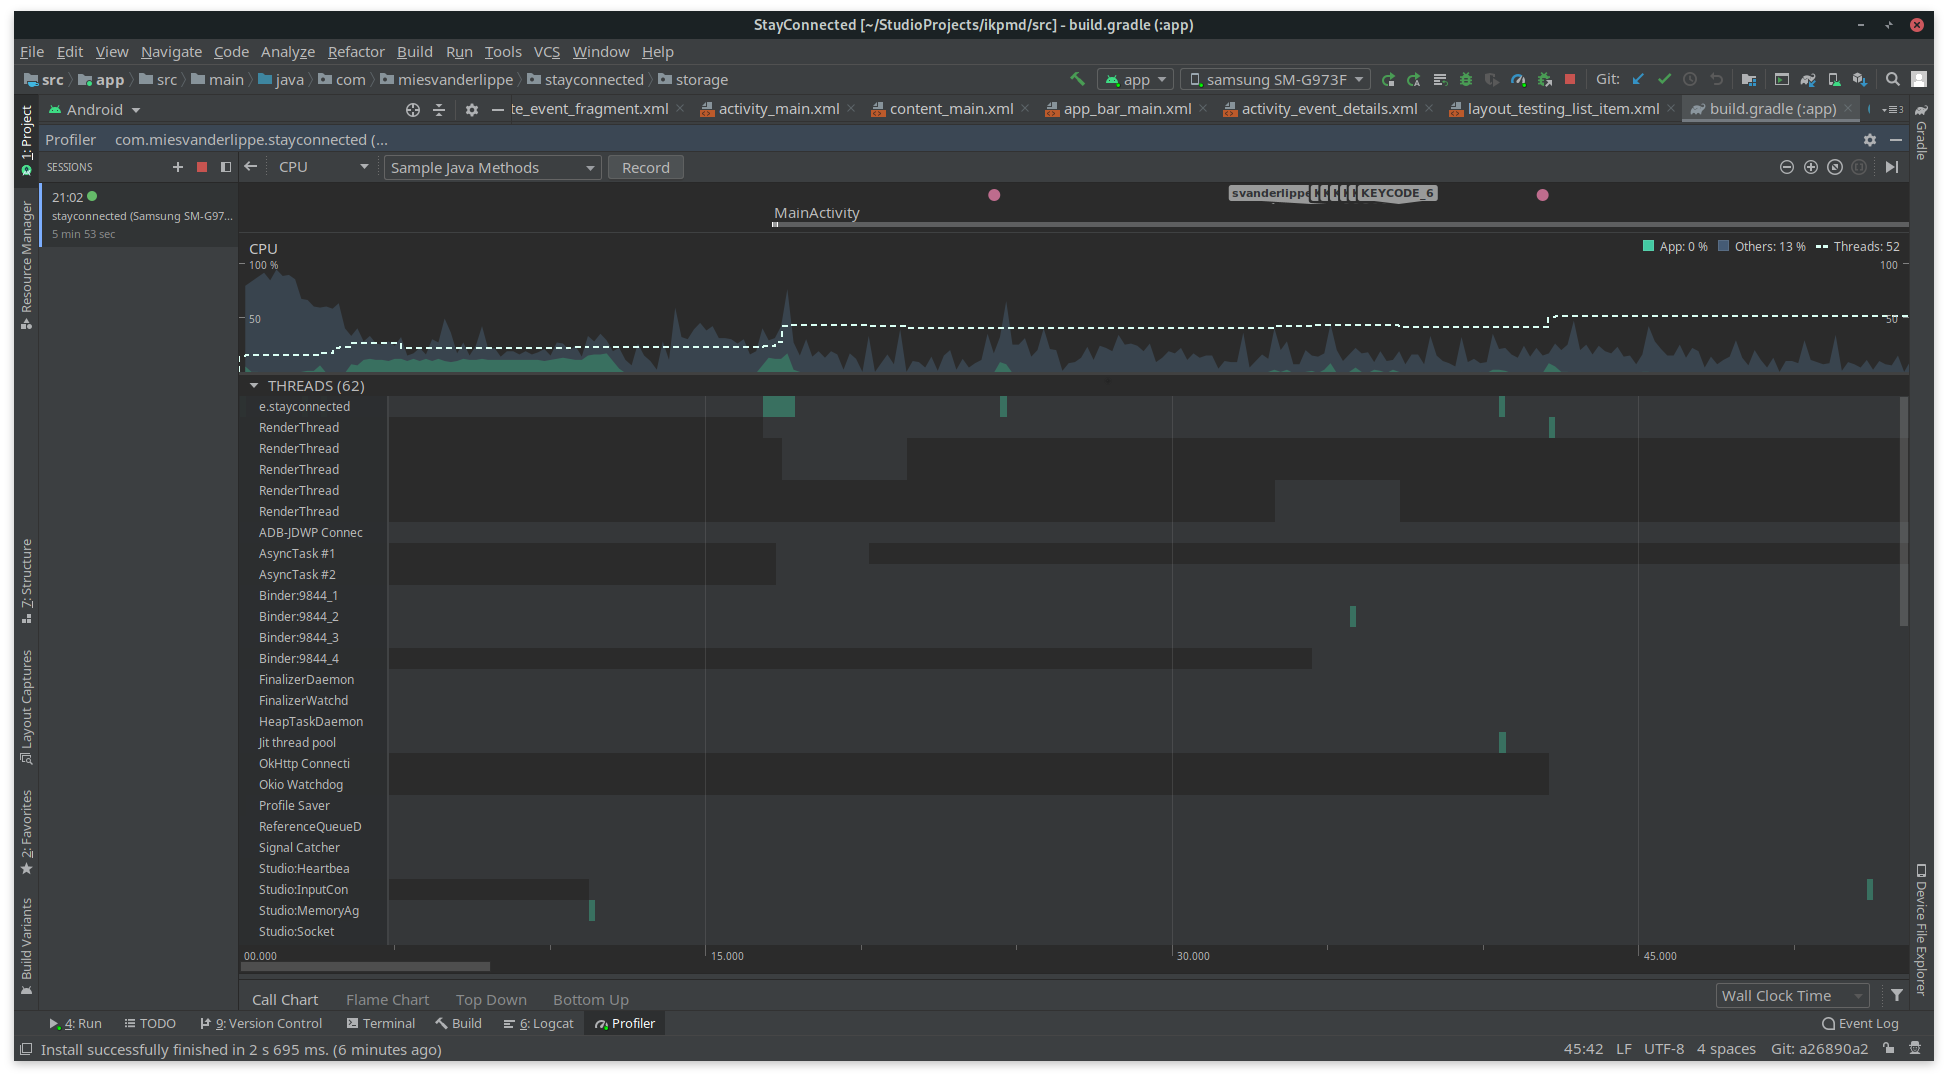
\includegraphics[width=0.95\linewidth]{images/CPUusage.png}
 		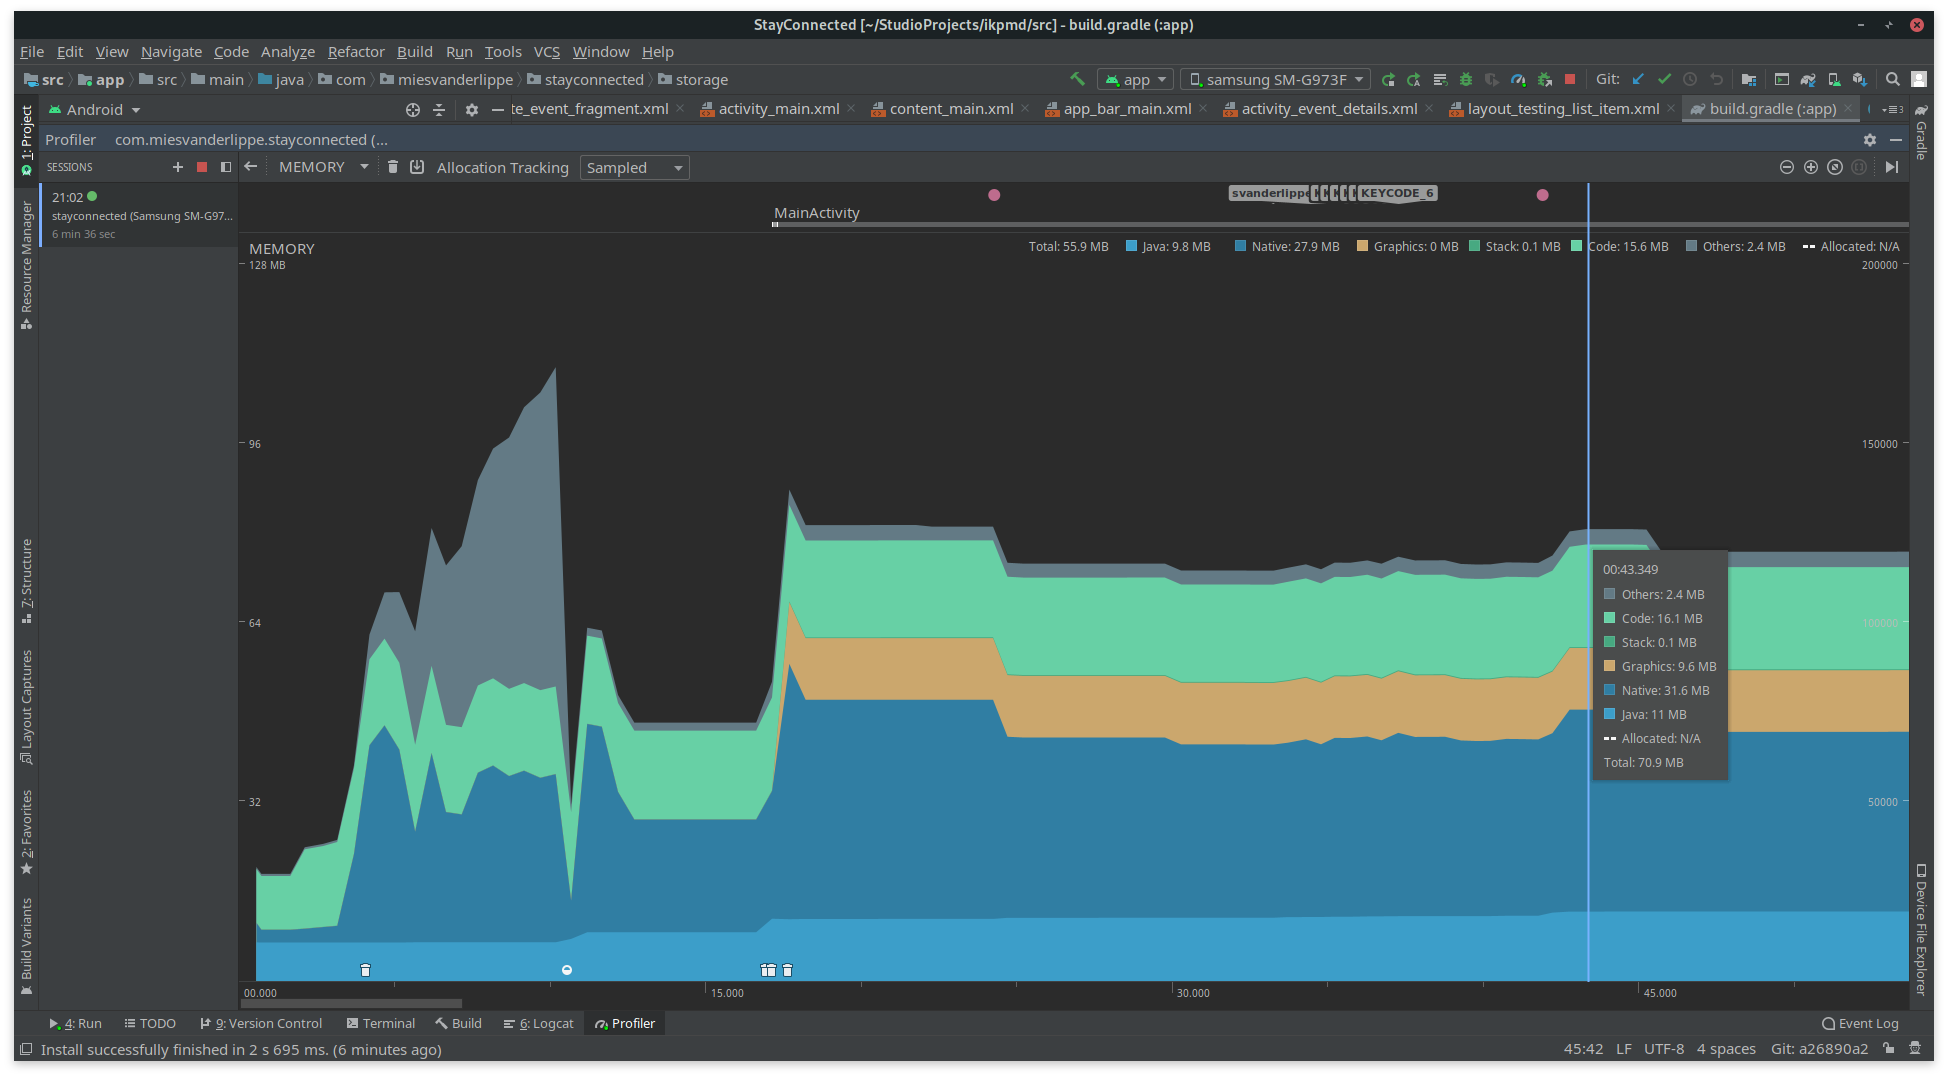
\includegraphics[width=0.95\linewidth]{images/RAMusage.png}
 		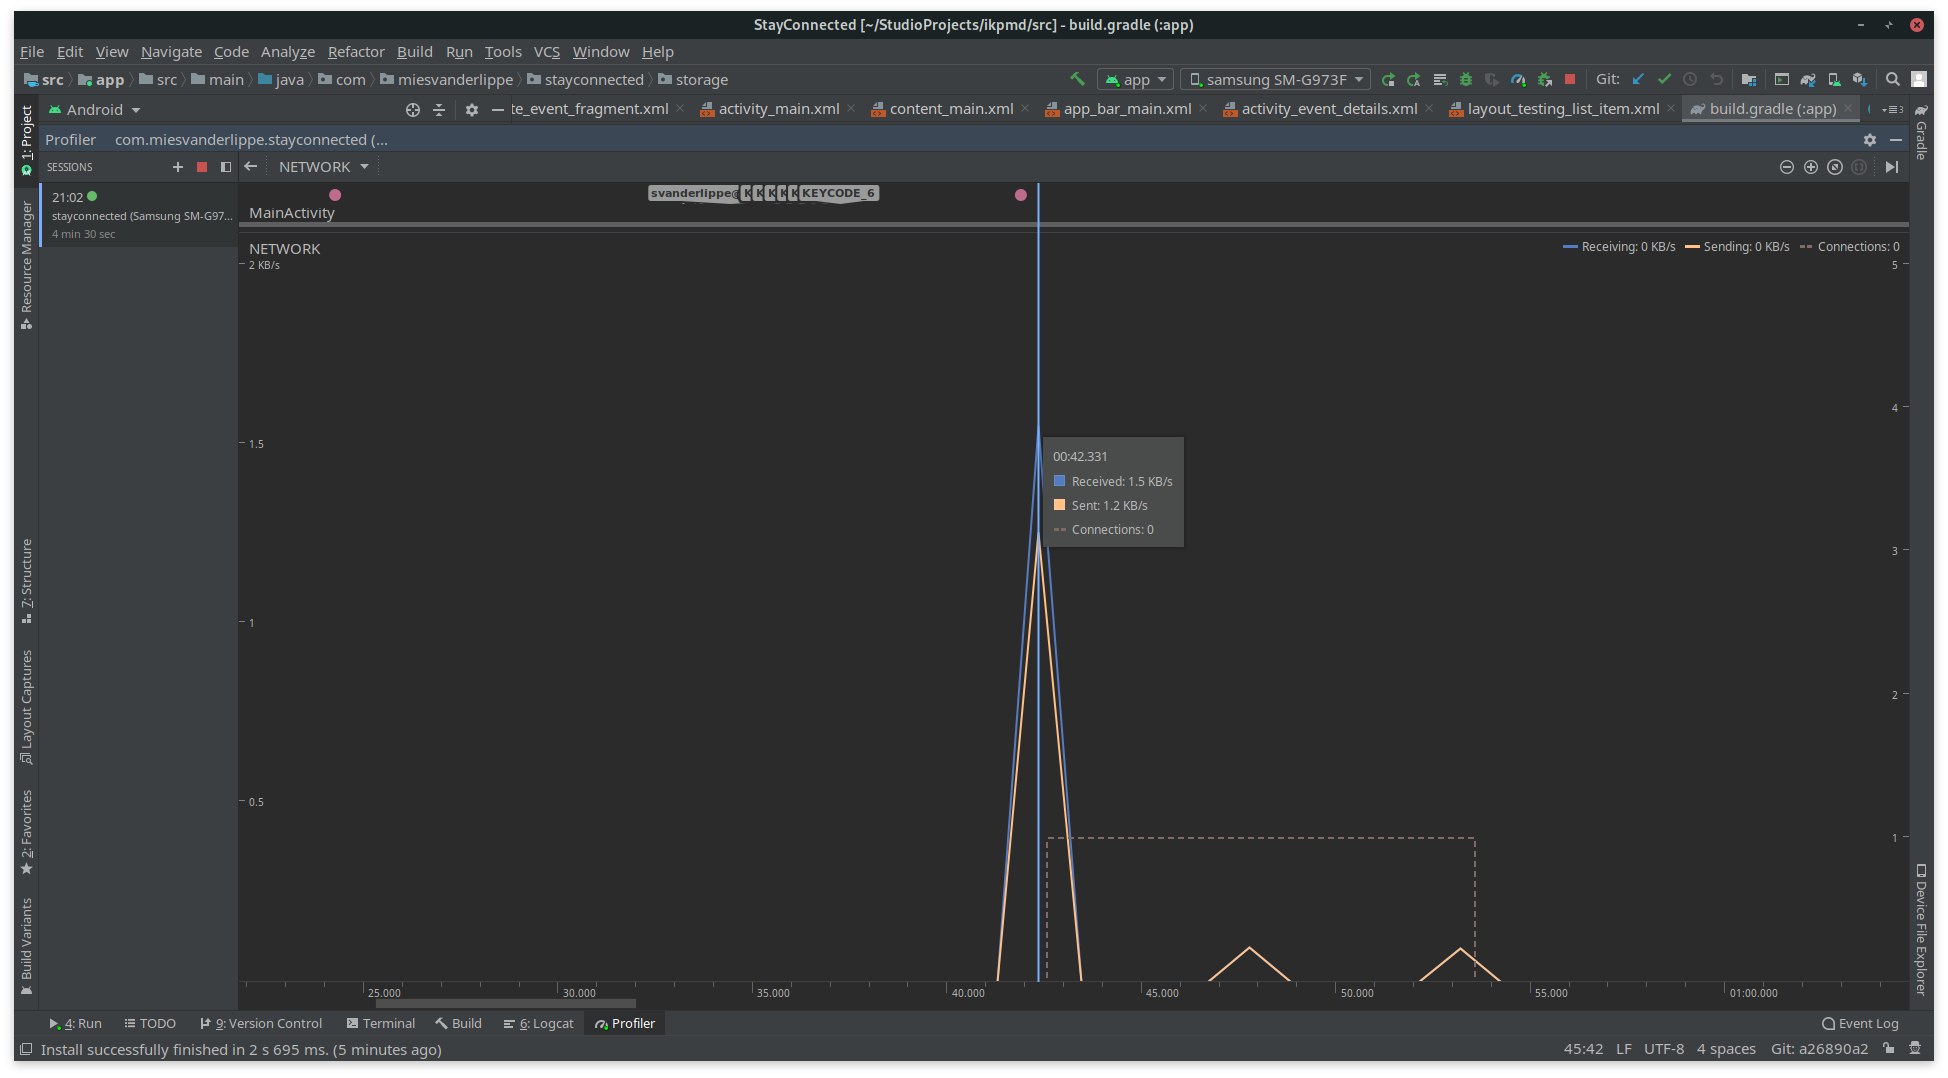
\includegraphics[width=0.95\linewidth]{images/dataUsage.png}
 	\end{center}
 	
	%% Een productverslag met screenshots van alle schermen. 
	%% Hier staat beschreven hoe de app werkt en welke (on)mogelijkheden de app heeft. Verder bevat het 
	%% productverslag o.a.op welke versie van de Android SDK is ontwikkeld,in hoeverre het MAVEN build 
	%% script is aangepast voor de applicatiemet een kleine uitleg, screenshots van de network statistics, 
	%% CPU-loaden memory usage opgenomen uit de DDMS.
		
	\newpage
	
	\section{Design}
	%% Een beschrijving van de gemaakte interface elementen, zoals buttons, invoervelden, toast msg 
	%% en/of snackbars. Er wordt een versie van een lijstgemaakt(bijvoorbeeld de ListView) Er wordt 
	%% gebruik gemaakt van parameter passing. Er wordt een manier van data visualisatiegemaakt om 
	%% gegevens inzichtelijk te maken.Tevens beschijf je kort hoe je material design hebt toegepast 
	%% in je app.
	
	
	\subsection{Het menu}
	Voor deze app is gebruik gemaakt van de app met menu template. In het menu worden de verschillende 
	mogelijkheden van de app getoond. Voor de account optie is een apart icoon gemaakt, voor de andere
	twee is gekozen voor iets dat in de buurt komt van een passend icoon en dat al in het template zat. 
	
	Zoals te zien is wordt de tekst bij het account aangepast als de gebruiker inlogt. 
	
	\begin{minipage}{0.50\textwidth}
		\begin{center}
			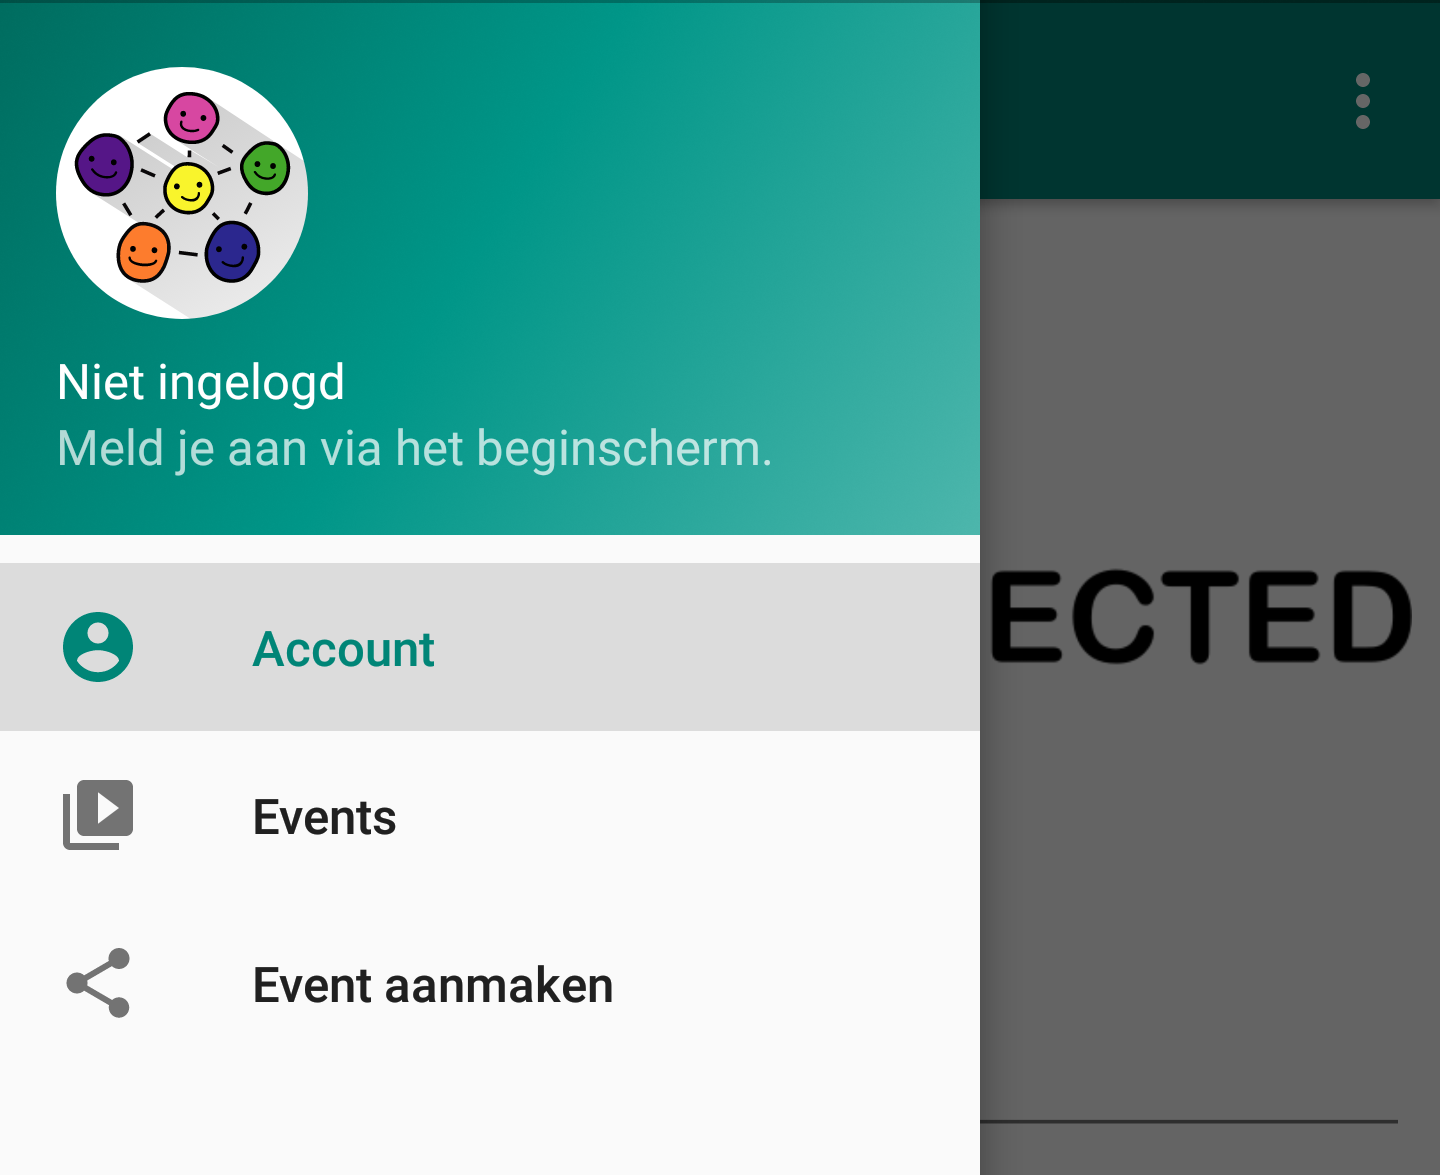
\includegraphics[width=5cm]{images/nietingelogd.png}		
		\end{center}
	\end{minipage}
	\hfill
	\begin{minipage}{0.50\textwidth}
		\begin{center}
			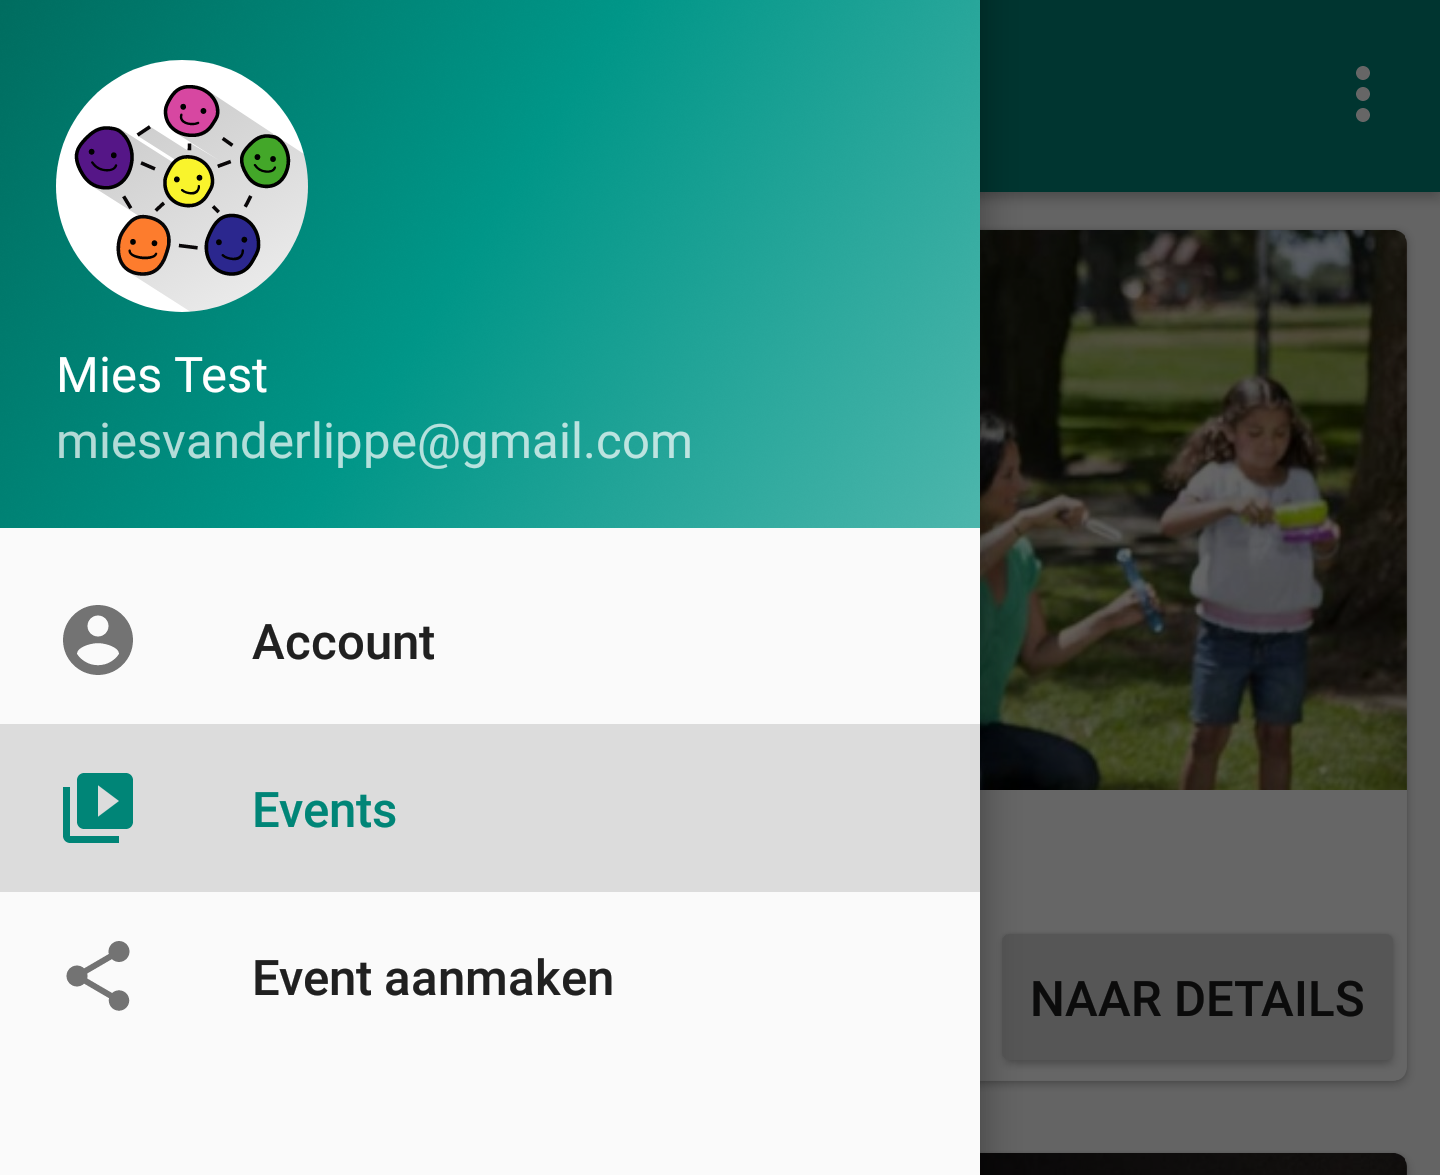
\includegraphics[width=5cm]{images/ingelogd.png}
		\end{center}
	\end{minipage}
	
	
	\subsection{De evenementen lijst}
	\begin{minipage}{0.60\textwidth}
	Een belangrijk design element in deze app is de lijst met kaartjes waarin de evenementen weergegeven
	worden. De combinatie van een afbeelding, tekst en knop geven veel ruimte voor het toepassen van de 
	richtlijnen en grafische elementen. 
	
	Zoals te zien is heeft de kaart een kleine 'hoogte' om zo een ruimtelijk effect te geven. De hoeken 
	zijn enigszins afgerond zonder dat het kitscherig wordt. De afbeelding vult het kaartje tot aan de 
	rand, wat rustiger is dan een randje eromheen laten. 
	
	Technisch is het een RecyclerView met daarin Cardviews, een RelativeLayout, een ImageView, wat 
	teksten en een knop.
	
	\end{minipage}
	\hfill
	\begin{minipage}{0.35\textwidth}
	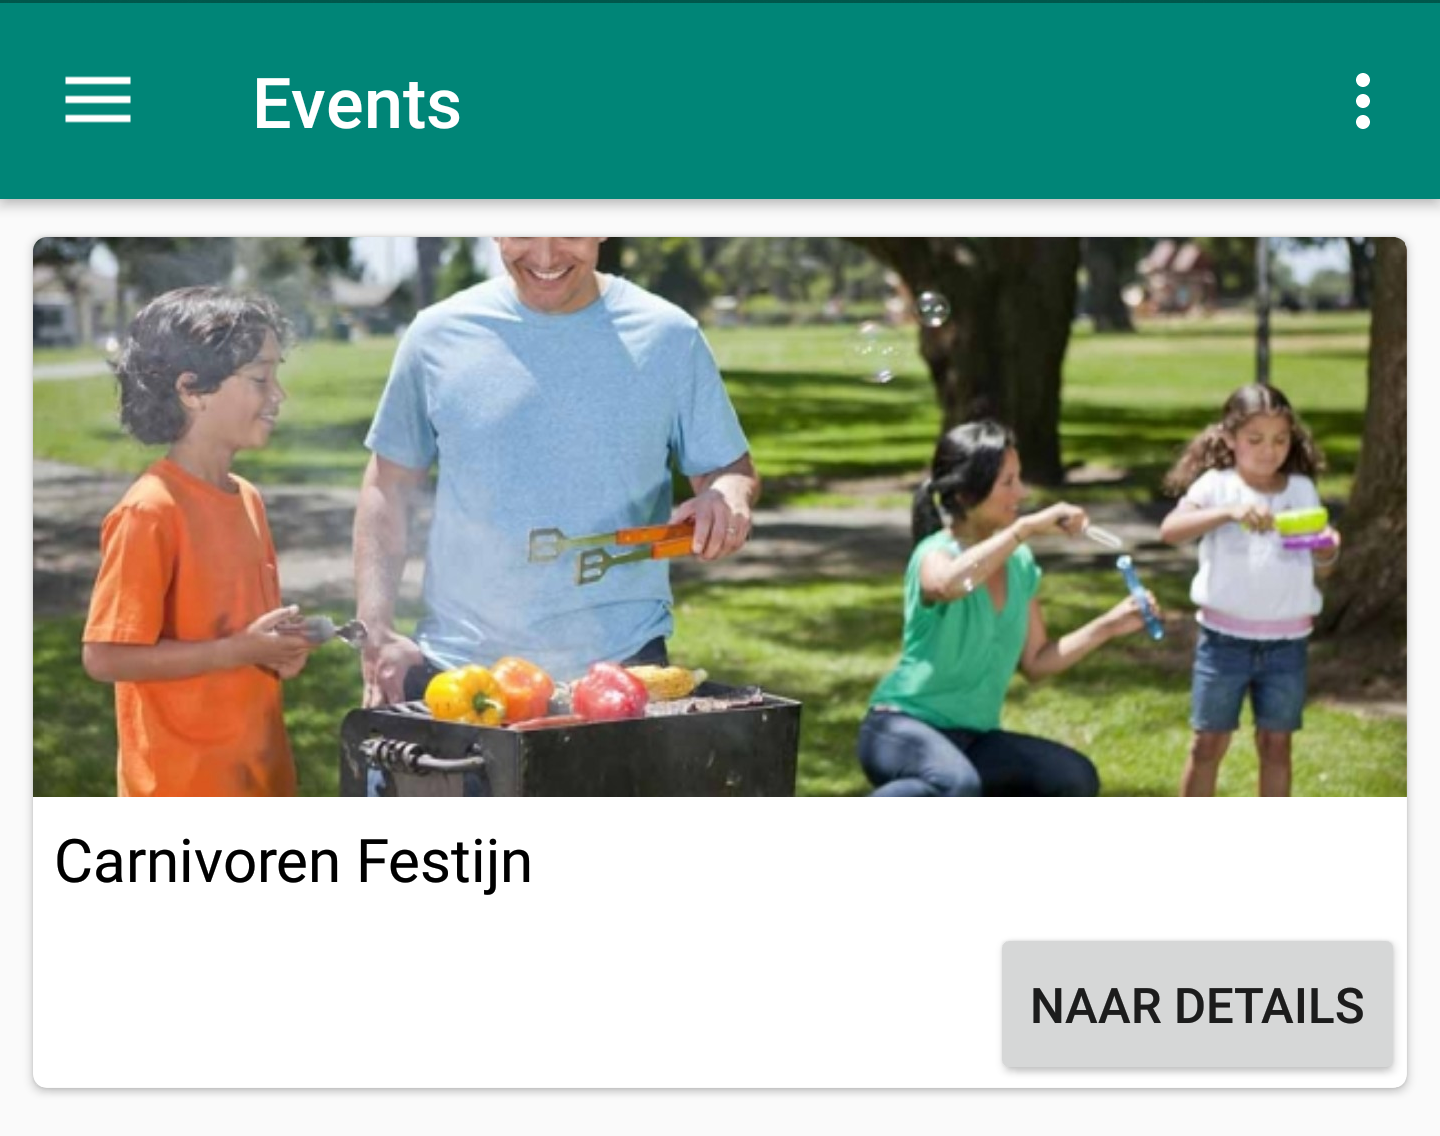
\includegraphics[width=\linewidth]{images/cardlist.png}
	\end{minipage}
	
	\subsection{Het account}
	Een gebruiker kan in- en uitloggen. Hier wordt gebruik gemaakt van de hints in de tekstinvoer. Voor 
	de rest is het een vrij eenvoudige layout. 
	
	\begin{minipage}{0.50\textwidth}
		\begin{center}
			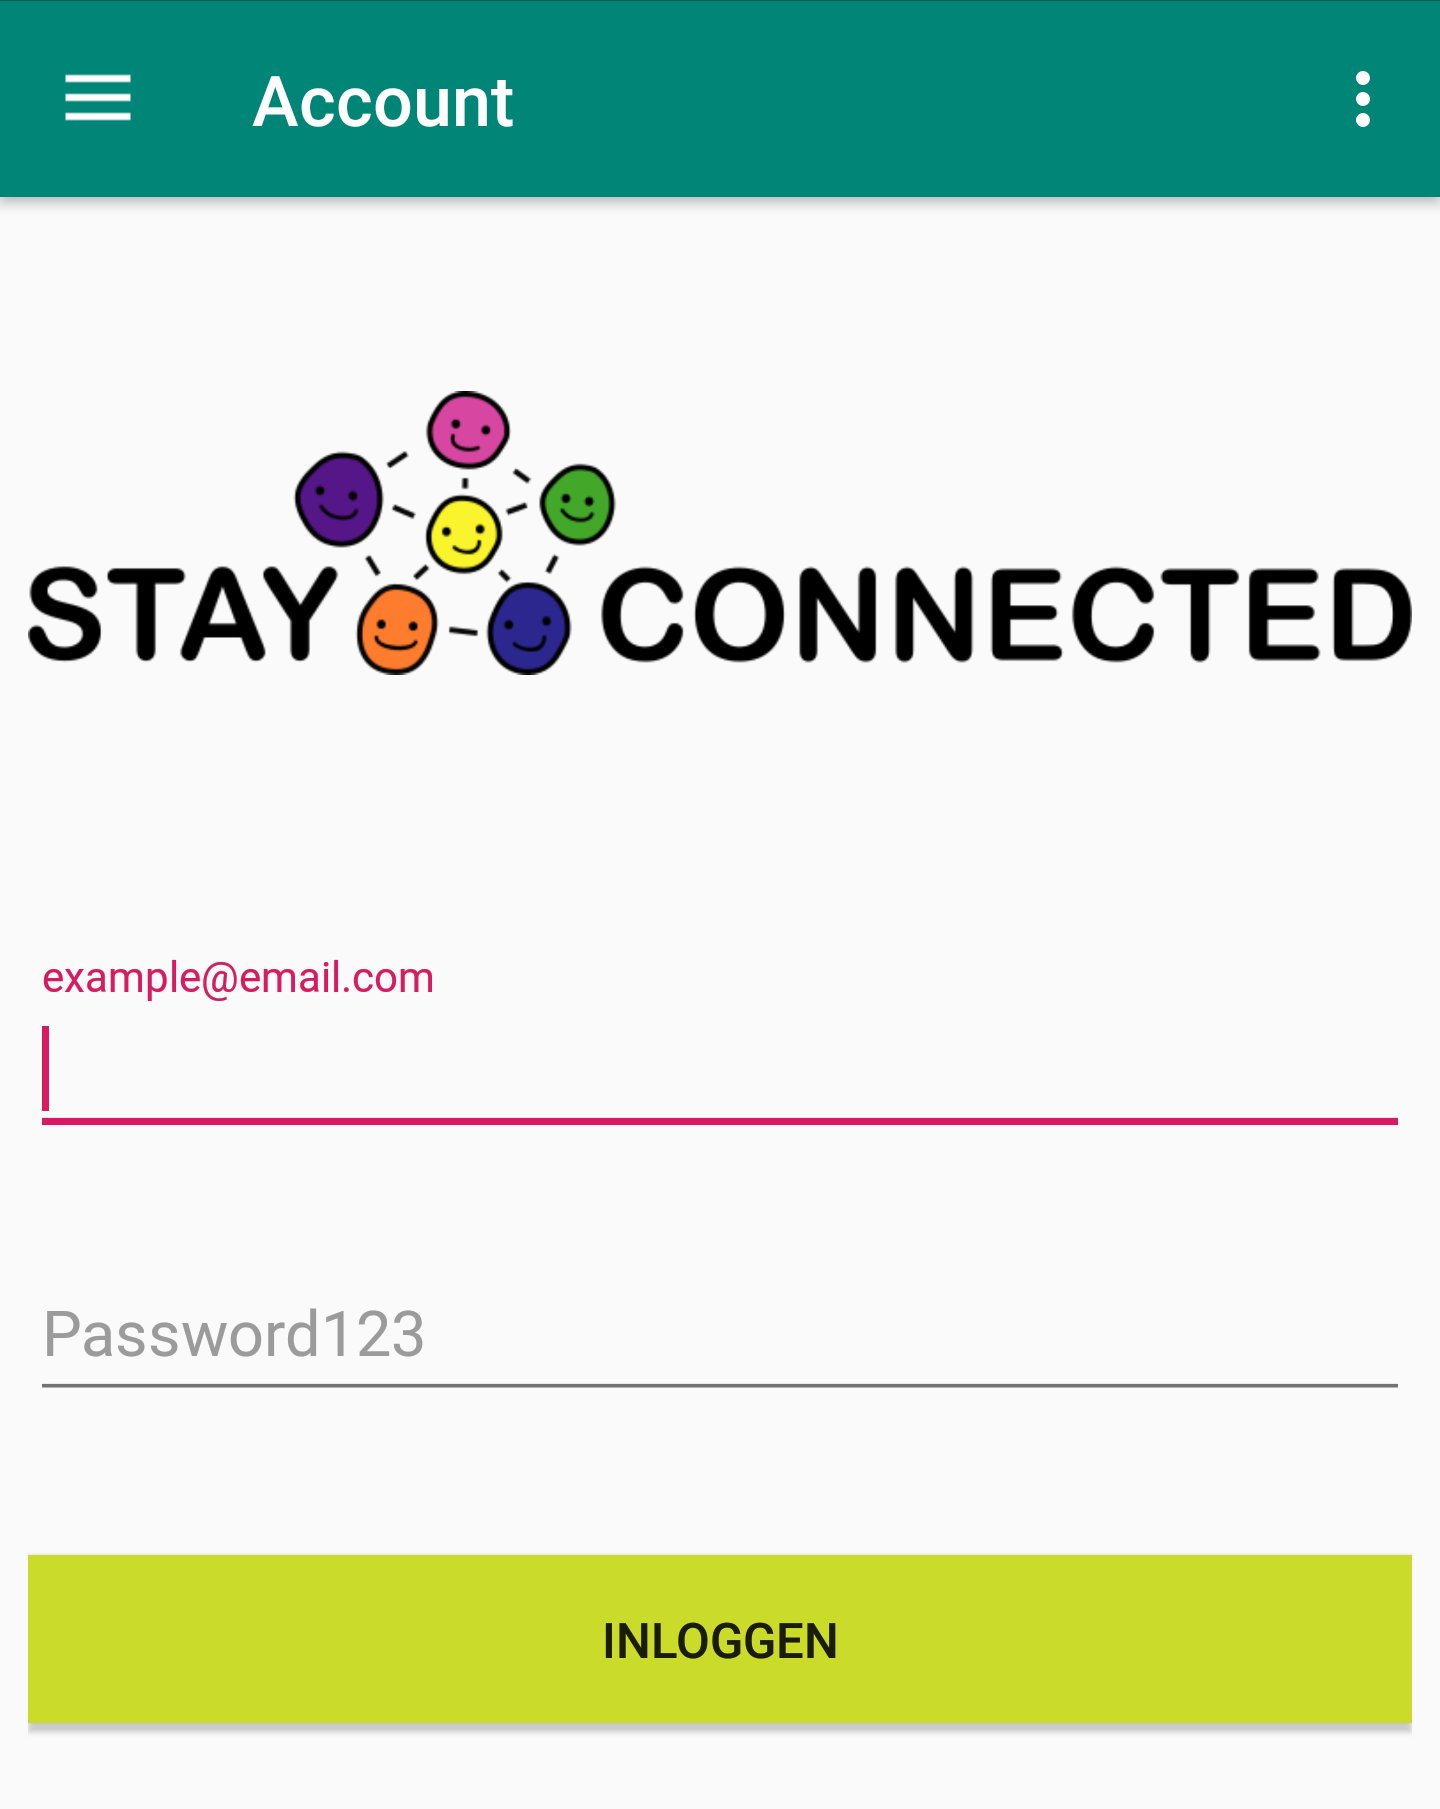
\includegraphics[width=5cm]{images/inloggen.png}		
		\end{center}
	\end{minipage}
	\hfill
	\begin{minipage}{0.50\textwidth}
		\begin{center}
			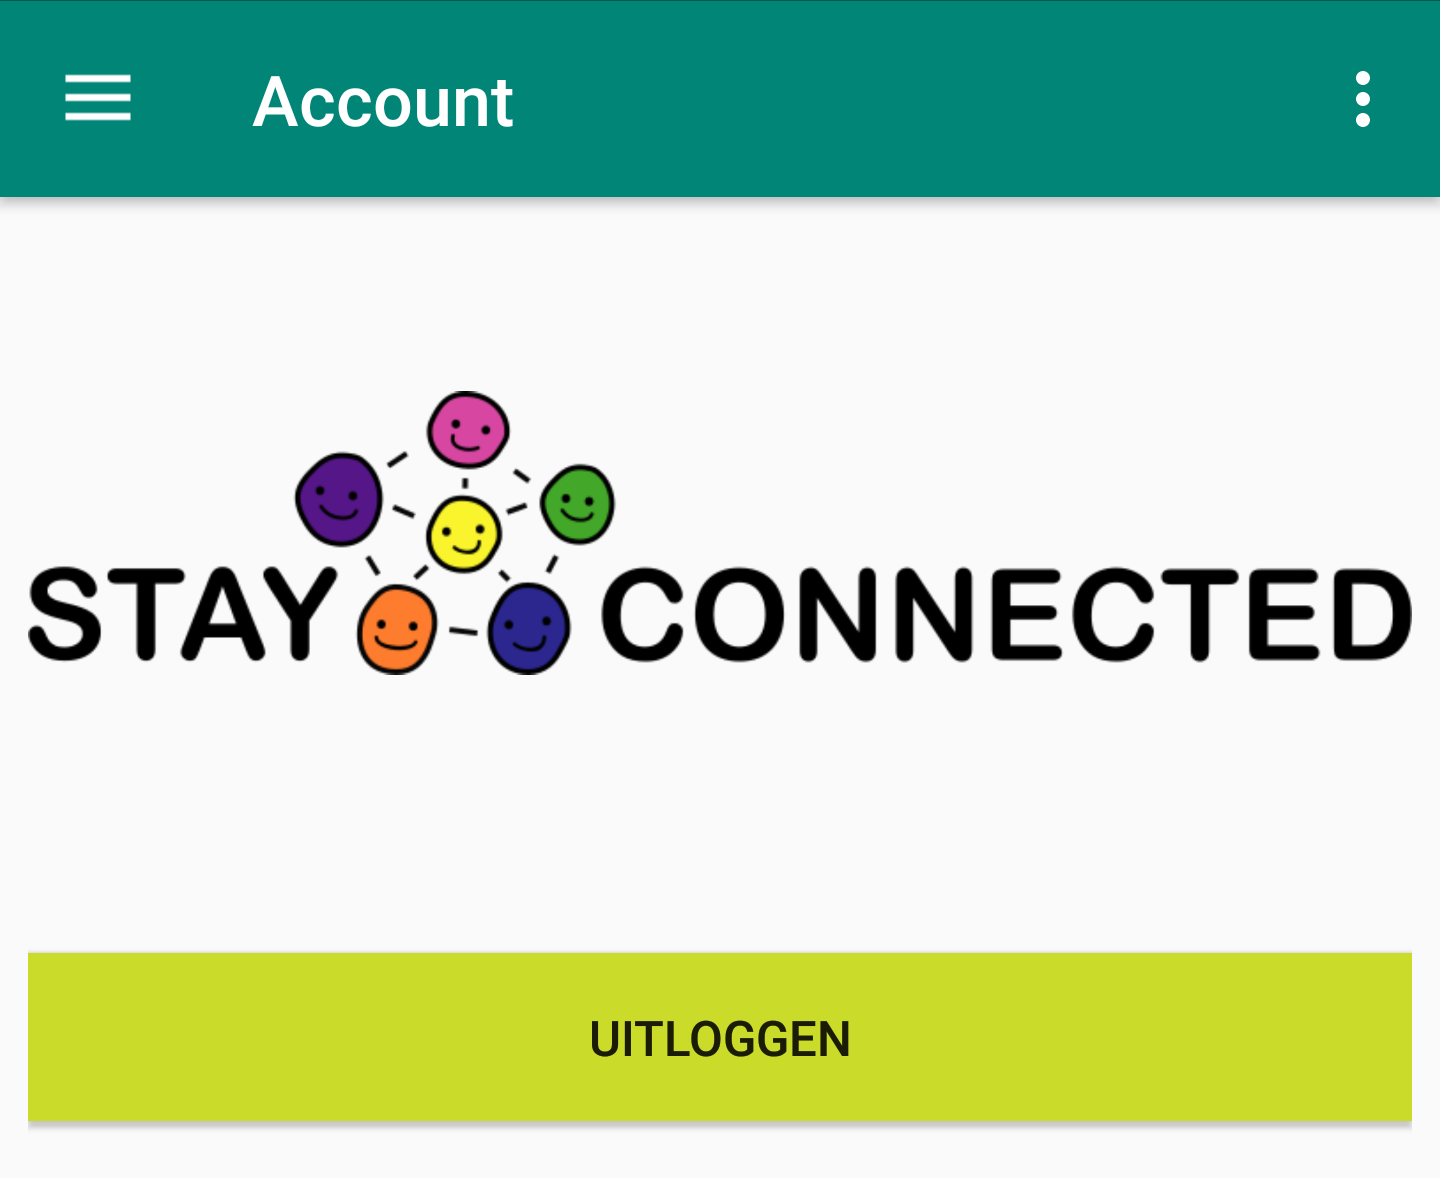
\includegraphics[width=5cm]{images/uitloggen.png}
		\end{center}
	\end{minipage}
	
	
	\subsection{De detailpagina}
	\begin{minipage}{0.60\textwidth}
	Een gebrek aan design is ook design toch? Voor de detailpagina is gekozen voor een robuste, eenvoudige
	weergave. Voor de deelname knop wordt na het laden de status van inschrijving opgehaald. Op basis daarvan
	wordt het een deelnemen- of verlaten- knop. De knop wordt dus ook verborgen voor niet ingelogde gebruikers
	of wanneer er geen verbinding is. Ook de balk bovenin is weggelaten omdat het idee is dat deze informatie
	over de app heen ligt. Als de inhoud te lang wordt, kan de gebruiker scrollen. 
	
	Deze weergave bevat vooral informatie uit het EventData object. Deze wordt geserializeerd en meegegeven 
	via de intent informatie bundel. De informatie over deelname wordt naderhand opgehaald aan de hand van 
	centraal geregelde informatie over de ingelogde gebruiker, en een repository voor evenementen. 
	
	\end{minipage}
	\hfill
	\begin{minipage}{0.35\textwidth}
		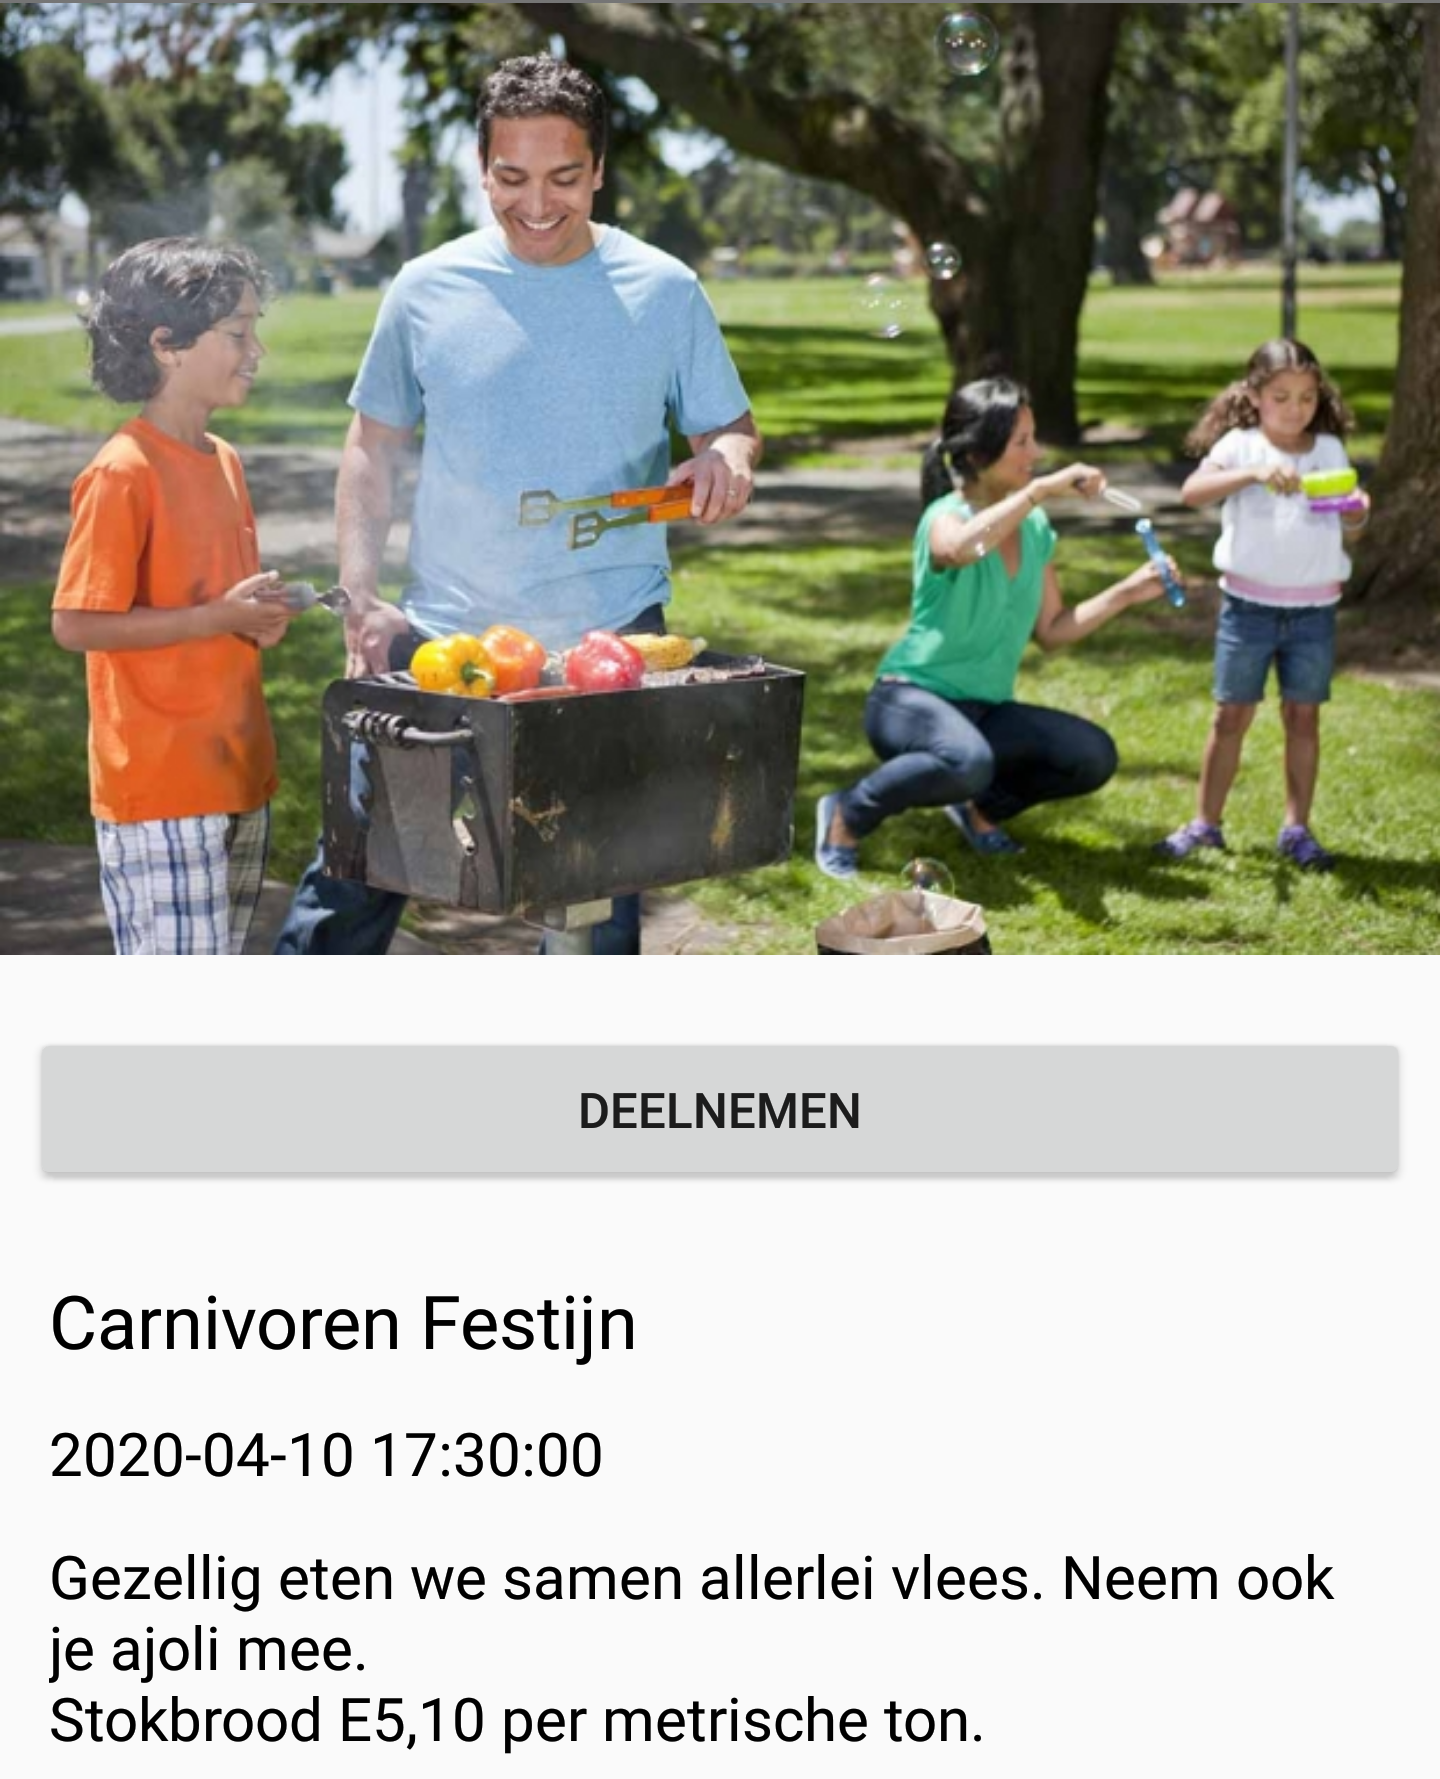
\includegraphics[width=\linewidth]{images/detailview.png}
	\end{minipage}
	
	\subsection{Het icoon}
	Voor de app is zowel een schaalbaar icoon gemaakt als een set 'ouderwetse' iconen. Met het gekke vector
	formaat dat Android gebruikt is dit niet even gemakkelijk. 


	\begin{minipage}{0.50\textwidth}
		\begin{center}
			
\includegraphics[width=2cm]{images/ic_launcher_round.png}
		\end{center}
	\end{minipage}
	\hfill
	\begin{minipage}{0.50\textwidth}
		\begin{center}
			
\includegraphics[width=2cm]{images/ic_launcher.png}
		\end{center}
	\end{minipage}	
	

	
	\section{De backend}
	%% Er is een beschrijving van de backend. Welke calls kan de API afhandelen, hoe werkt de API, waar 
	%% wordt de data opgeslagen. Waarom is er gekozen voor deze manier van dataopslag?Dit onderdeel mag 
	%% ook de beschrijving van de Firebase toepassing zijn.Er moet een vorm van persistente dataopslag 
	%% gemaakt worden.Tevens beschrijf je in hoeverre de app off-line kan werken.Het beschrijvenvande 
	%% backend, het lezen uitde backenden het schrijven naar de backend zijn onderdelen van de opdracht
	
	\subsection{De API}
	De API is een voor dit project zelfgebakken achterkant van de website van StayConnected. Voor dit 
	project draait deze een aparte kopie met een eigen database. Alle functies hebben een API key nodig.
	Deze is voor nu gewoon een pre-shared key die in de app gebakken zit. Niet de meest veilige optie, 
	maar het is dan ook maar een schoolproject. Daarbij zijn de gegevens die hiermee inzichtelijk zijn 
	sowieso publiek. 
	
	Naast de api key die met alle requests meegestuurd moet worden, is er ook een persoonlijke token. Deze
	kan opgevraagd worden via de API en werkt in combinatie met het e-mail adres van de gebruiker. Allebei
	deze gegevens worden dan dus ook opgeslagen in de app via de private gegevens API van Android. 
	
	Het ondersteunt de volgende functies (de functie wordt aangegeven met de get parameter) :
	\begin{enumerate}
		\item events\\
		Een lijst met evenementen. 
		
		\item get\_participation\\
		POST/GET: activity\_id (Het ID van het evenement)\\
		POST/GET: email (De e-mail van de gebruiker)\\
		POST: token (De persoonlijke token van de gebruiker.)\\
		Vraagt de deelname van een gebruiker op. Komt in een simpel model met alleen de waarde 'participates' 
		
		\item set\_participation\\
		POST: event-id (Het ID van het evenement)\\
		POST: email (De e-mail van de gebruiker)\\
		POST: token (De persoonlijke token van de gebruiker.)\\
		POST: participates (bool, of een gebruiker deel zal nemen)\\
		Geeft de deelname van een gebruiker aan. Geeft de nieuwe status terug zoals get\_participation doet. 
		
		\item get\_token\\
		POST: email (De e-mail van de gebruiker)\\
		POST: password (Het wachtwoord van de gebruiker.)\\
		Geeft o.a. een token terug. Alle volgende waardes zitten in de response: success, admin, token, 
		user\_model, message. Het user model bevat wat overige informatie van de gebruiker zoals het e-mail adres.
		
		\item create\_event\\
		POST: email (De e-mail van de gebruiker)\\
		POST: token (De persoonlijke token van de gebruiker.)\\
		POST: name-event (De naam van het evenement)\\
		POST: location-event (De locatie waarop het evenement plaatsvind)\\
		POST: desc-event (De omschrijving van het evenement)\\
		POST: date-event (De datum waarop het plaatsvind jjjj-mm-dd uu:mm:ss)\\
		POST: image-event(Een begeleidende, om-en-nabij vierkante afbeelding)\\
		Maakt een evenement aan en reageert met een status. 
		
	\end{enumerate}

	\subsection{Caching}
	De evenementen worden opgeslagen in een lokale SQLite database. Hierover is meer te vertellen onder 
	'\nameref{eigen-inbreng}'. Het e-mail adres en de token worden opgeslagen in de Shared Preferences, 
	met de private context uiteraard. Inschrijving wordt niet bijgehouden. 
	
	Wanneer een gebruiker bezig is met een evenement aanmaken en de app sluit, wordt dit ook opgeslagen 
	in shared preferences. Hiervoor is gekozen, omdat het weinig data betreft en geen collectie betreft. 
	Had de app ook evenementen kunnen aanpassen, dan had het misschien logisch geweest een tabel bij te 
	houden van alle huidige aanpassingen.  
	
	Voor beiden is een abstractie laag geschreven. Die van de gebruikers gegevens is te vinden onder 
	login.CheckLogin en die voor evenementen is verdeeld over data.StayConDatabase, entities.EventEntity,
	repositories.EventRepository en repositories.RemoteEventRepository. 
	
	\subsubsection{Offline werken}
	De app kan dus off-line een evenement aanmaken en de bestaande evenementen weergeven. Alle andere
	functionaliteiten vereisen een internetverbinding, want dat is inherent aan de opstelling. 
	
	\subsection{Werken met de abstracties}
	De gebruikersgegevens kunnen opgehaald worden via een instantie van login.CheckLogin. Deze klasse
	kent de functies getUserToken, getUserName, getUserEmail die allemaal doen wat er op het doosje staat. 
	De enige kanttekening is dat de functies de string "None" teruggeven als er geen gegevens beschikbaar
	zijn. 
	
	Het gebruiken van de evenementen repository vereist wat meer uitleg. Dit code voorbeeld komt uit 
	ui.events.EventsFragment. 
	
	\begin{lstlisting}
val dao = StayConDatabase.getDatabase(view.context).eventDao()
eventRepository = EventRepository(viewLifecycleOwner, view.context, dao)

val adapter = EventsRecyclerViewAdapter(view.context)

eventRepository!!.allEvents.observe(viewLifecycleOwner, Observer { 
	allEvents ->
	// Update the cached copy of the words in the adapter.
	allEvents?.let {eventEntityList ->
		adapter.updateEvents(eventEntityList.map { event ->
				EventData(event.id, event.activityName, 
				event.location, event.description, 
				event.dateTime, event.imageUrl
			)
		})
	}
})

eventRepository!!.queueRefresh()

	\end{lstlisting}
	
	De dao is een abstractie object van de database. Hierin liggen een reeks queries vastgelegd. Deze wordt
	meegegeven aan de EventRepository, welke de offline collectie beheerd, en de online collectie op kan vragen. 
	De allEvents lijst is in de eerste momenten dat de klasse geinitialiseerd wordt leeg. Op dat moment wordt 
	asynchroon de data uit de lokale cache opgehaald. Hierom 'observen' we de collectie en werken we de collectie
	in de adapter bij. Er vind ook nog wat mapping plaats tussen de objecten zoals die in de API gebruikt worden, 
	en zoal die in de cache staan want dat verschilt. Dan wordt er ook nog een refresh opgevraagd wat ook 
	a-synchroon gebeurt. Als de refresh klaar is wordt opnieuw de observer aangeroepen en update de recyclerview 
	automatisch. Dit betekend dus ook dat als de gebruiker offline is, of traag internet heeft deze alsnog direct
	een gevulde view te zijn krijgt. 
	
	\section{Eigen inbreng}\label{eigen-inbreng}
	%% Eigen toevoeging aan de app. Een onderdeel wat niet in de les is besproken, maar welke de student 
	%% zelf heeft uitgezocht. Wat dat onderdeel doet, inclusief bronvermelding, wordt kort besproken. 
	%% Dit kunnen bijvoorbeeld zijn;hamburger menumaken, gebruik van fragments, animaties, externe 
	%% libraries gebruiken e.d.Als je wireframes hebt gemaakt voor het ontwerpen van je app mag je deze 
	%% ook aanleveren.
	\subsection{De basis app}
	Deze app maakt gebruik van een Drawer Menu Activity. Dit betekent dat alle inhoud verstopt zit in fragments
	en dat dus enig tutorial niet zonder aanpassingen werkt. Hieraan zijn eigen fragments toegevoegd, is een 
	app-icoon voor gemaakt en is eigenlijk alle inhoud aangepast. 
	
	\subsection{Kotlin}
	Deze app is ook niet geschreven in Java. In plaats daarvan is er  - in overleg -gekozen om Kotlin te gebruiken. 
	Dit, omdat deze taal wat modernere syntax kent en Mies een verwent en eigenwijs C\# programmeur is.

	\subsection{androidx.room}
	Een andere eigenwijsheid is het absoluut zo min mogelijk willen schrijven van queries. Of het in dit project 
	tijd bespaard heeft? Waarschijnlijk niet. 
	
	Room is een framework waarin op een keurige manier de data gescheiden wordt van de bron. Het bied enkele 
	abstracties van de database zelf, een architectuur voor het aanleveren van data en systemen voor het 
	inregelen van de lifetime van de data. Het doel van Room is o.a. caching waar het in dit project voor gebruikt 
	is. 
	
	\vspace{1em}
	Deze uitleg en tutorial is gevolgd: https://codelabs.developers.google.com/codelabs/android-room-with-a-view-kotlin/
	
	\subsection{Eigen drawables}
	Vanuit SVG's is er voor dit project een schaalbaar app-icon gemaakt en een custom icoon voor in het menu gemaakt.
	Hiervoor is ook de ingebouwde 'Asset Studio' gebruikt wat eigenlijk meer een veredelde import is.
	
	\subsection{De gehele API}
	Voor dit project is ook een API geschreven in PHP. Deze praat met een bestaande database om de gegevens door te geven. 
	De development website is ook beschikbaar op: 
	
	http://stay-connected.miesvanderlippe.com/
	
	Deze pagina geeft ook dezelfde gegevens weer als die in de app zichtbaar zijn. 
	
	\subsection{Afbeeldingen uploaden}
	Standaard is het best lastig om een afbeelding te uploaden. Om dit toe te staan is gebruik gemaakt van een custom 
	request dat multi-part data ondersteund: 
	
	https://medium.com/better-programming/how-to-upload-an-image-file-to-your-server-using-volley-in-kotlin-a-step-by-step-tutorial-23f3c0603ec2
	
	
	\section{Git}
	%% De link naar de GIT repository met een beschrijving van de gebruikte branches. 
	De Git repository is hier te vinden: 
	
	https://github.com/miesvanderlippe/ikpmd
	
	\begin{itemize}
		\item master\\
		Hier staan alle functies die af zijn in. 
		\item better-event-details\\
		Gebruikt om een mooiere detailpagina te maken, en voor inschrijven
		\item caching-events\\
		Hierin is de caching met Room gemaakt
		\item card-list-activity\\
		Een van de eerste branches, betreft de kaartjes weergave
		\item docs\\
		Documentatie branch. Wordt gemerged aan het einde van het project. 
		\item exercises-mies\\
		De oefeningen die Mies gemaakt heeft tijdens de les. 
		\item improving-code \\
		Tussen het implementeren door moesten wat kleine wijzigingen gemaakt worden. Deze hadden geen betere plek. 
		\item login-screen\\
		Het login scherm. 
		\item photo\_upload\\
		Hierin is het uploaden van foto's ontwikkeld.
	\end{itemize}
	
	\section{Bronnenlijst}
	%% Bronnenlijst van alle gebruikte websites, literatuur en andere bronnen
	Het implementeren van Room caching: 
	https://codelabs.developers.google.com/codelabs/android-room-with-a-view-kotlin/
	
	Bestanden uploaden via HTTP
	https://medium.com/better-programming/how-to-upload-an-image-file-to-your-server-using-volley-in-kotlin-a-step-by-step-tutorial-23f3c0603ec2
	
	SharedPreferences referentie
	https://developer.android.com/reference/android/content/SharedPreferences
	
	Het instellen van een naam bij het uitklappen van het menu
	https://developer.android.com/reference/android/support/v4/widget/DrawerLayout.DrawerListener
	
	Live collecties
	https://developer.android.com/topic/libraries/architecture/livedata.html
	
	\newpage
	\section{Individueel}
	
	\subsection{Roel}

	\subsubsection{Aandeel in de app}
	Bij het maken van de app heb ik me bezig gehouden met het maken van een aantal elementen. Deze zijn:
	\begin{enumerate}
		\item De backend class van het loginscherm.
		\subitem FetchKey en CheckLogin
		\item Het opslaan van login gegevens die terug gegeven worden door de API.
		\subitem DataStorage
		\item Een deel van de backend class voor het maken van een nieuw event.
		\subitem Het Event model en deel van de POST request.
		\item Het cachen van een event wanneer deze niet volledig/succesvol is aangemaakt.
		\subitem CreateEventCache
	\end{enumerate}
	% De student beschrijft welke delen van de app door hem/haar gemaakt zijn.Dit is terug te vinden in de branches van de GIT-omgeving
	\subsubsection{Reflectie op de samenwerking}
	Voor mijn gevoel ging de samenwerking vrij soepel, hoewel het soms lastig is om bepaalde concepten over te dragen via chat berichten. Ook is mijn programmeer kennis vrij gelimiteerd en heb dus veel gestruikeld over soms triviale dingen. Gelukkig is Mies erg ervaren in verschillende programmeer talen, om deze reden heeft hij mij vaak bij de hand kunnen nemen en dingen op te lossen als ik er niet meer uit kwam. Mijn conclusie is dan ook, dat ik genoten heb van de samenwerking.
	\subsubsection{Aanbeveling}
	Over het algemeen vond ik de module vrij goed ingericht. Vooral omdat je uiteindelijk aardig wat vrijheid hebt met het ontwikkelen van de eind-app. Wat wel leuk zou zijn, is de keuze vanaf het begin om met Kotlin te werken in plaats van Java. Deze switch is ook niet al te moeilijk, sinds Android Studio Java zelf kan converteren naar Kotlin.
	% Aanbeveling over de module op inhoudelijk gebied: de student adviseert welke onderwerpen van applicatieontwikkeling moeten blijven 
	% in het aangeboden onderwijs en welke onderwerpen wenselijk zijn die niet zijn aangeboden, inclusief relevante verwijzingen naar
	% ondersteunende artikelen
	
	\subsection{Mies}

	\subsubsection{Aandeel in de app}
	% De student beschrijft welke delen van de app door hem/haar gemaakt zijn.Dit is terug te vinden in de branches van de GIT-omgeving
	Ik ben de app begonnen met het ontwikkelen van de lijst van kaartjes. Roel heeft de eerste implementatie gemaakt waarin JSON data 
	van de API opgehaald werd en ik heb die weer omgebouwd naar caching. Roel heeft de opzet gemaakt van het aanmaken van het evenement
	en ik heb die UI herschreven en een probleem opgelost met het versturen van de data. Veel elementen zijn opgezet door mij en afgemaakt
	door Roel, of andersom. Immers moesten we er allebei van leren en liepen we allebei tegen problemen aan. 
	
	Ik ben helemaal verantwoordelijk voor de PHP API en Roel is geheel verantwoordelijk voor de SharedPreferences. 
	\subsubsection{Reflectie op de samenwerking}
	% Reflectie over de samenwerking en het leerproces van de student
	Dit is niet zonder reden het zoveelste project dat ik met Roel samen doe. Hij is een betrouwbare groepsgenoot waarvan ik goed weet wat
	hij goed kan, en waar ik hem kan helpen. Roel is beter dan ik in gewoon doorwerken, en ik heb wat meer ervaring met programmeren.
	
	Ik kan hier nog tal van rozen, kruizen en situaties omschrijven. Of dat wat toevoegd? Ik betwijfel het. Roel verdient elke punt van 
	het eindcijfer.
	
	\subsubsection{Aanbeveling}
	% Aanbeveling over de module op inhoudelijk gebied: de student adviseert welke onderwerpen van applicatieontwikkeling moeten blijven 
	% in het aangeboden onderwijs en welke onderwerpen wenselijk zijn die niet zijn aangeboden, inclusief relevante verwijzingen naar
	% ondersteunende artikelen
	Android ontwikkeling is redelijk overzichtelijk als gehouden wordt aan simpele activities en intents. In dit project zijn Roel en ik 
	zwaar van het vertrouwde spoor afgeweken en hebben daardoor misschien meer geleerd over complexere principes. Ik denk dat fragments,
	lifecycles en het inregelen van centrale repositories e.d. beter terug kan komen in de module. 
	
	Met wat uitleg ben ik ervan overtuigd dat de Room library waardevoller is dan hoe er nu omgegaan wordt met SQLite. Een query schrijven
	kan bijna iedereen op dit punt in de opleiding, maar gebruik maken van caching en abstracties is leuk en leerzaam. 
	
	Voor de rest heb ik uitgevonden dat je zeker op Unix systemen vrij gemakkelijk een live schermopname kan streamen. De configuratie is
	wat gevoelig, maar met onderstaand commando werkt het goed. Zo zou een demonstratie op afstand mogelijk worden. 

	\begin{lstlisting}
adb exec-out screenrecord --bit-rate=16m --output-format=h264 --size 1280x720 - |\
mplayer -framedrop -fps 6000 -cache 512 -demuxer h264es -
	\end{lstlisting}


\end{document}
